
\begin{document}

\chapter{Experimental Setup}

\label{chapter:experimentalsetup}

\section{Design}

In order to quantify the performance of the developed planner and to judge how
well it performs, experiments needed to be run that can determine the degree of
safety present in the generated paths and how long it takes to generate these
paths. To gather this data, three different scenes were created with differing
number dynamic obstacles with different trajectories. The independent
variables, or parameters, for each scene consisted of the amount of noise,
$\epsilon$ for the dynamic obstacles and the speed of the robot, $s$. For the
experiments, a given value of $\epsilon$ is the same for all of the dynamic
obstacles in the scene. The amount of noise ranges from $0.002$ to $0.01$ with
an increment of $0.002$ and the speed ranges from $1.0$ to $4.5$ meters per
second with an increment of $0.5$ meters per second. Due to the stochasticity
of the planner and the dynamic obstacles, each set of parameters for each scene
was run 20 times. The values for each metric recorded is averaged and the
standard deviation for each set of parameters for each scene is presented.

In order to judge how the developed planner compares to a standard algorithm
developed to plan in stochastic dynamic environments, a slight variant to the
potential fields planner described in Algo.~\ref{algo:pf} was implemented. The
difference is that the implemented potential fields planner used a different
repulsive potential function that is described in Eq.~\ref{eq:betterrep}.

\begin{equation}
    U_{\Var{rep}}(p, t, A) = \max_{a \in A} \,
    \frac{k}{||\tilde{\zeta_a}(t) - g||^2 + \varepsilon}
    \label{eq:betterrep}
\end{equation}

In Eq.~\ref{eq:betterrep}, $k$ is a scaling constant where $k > 0$, and
$\varepsilon$ is constant where $0 < \varepsilon < k$ that ensures that the
function does not exhibit a singularity. This variant in the potential fields
ensures that the planner has no information about the motion of the obstacles
and can thus be used to compare how this information can benefit a planner.
Also, since this planner is not sampling based, it can be used to see how a
complete sampling based planner can be more or less effective. The results from
this experimental setup are described in Ch.~\ref{chapter:results}.

\section{Metrics}

To quantify the performance of the planners, four metrics are used, three to
measure the safety and one for computational time. Along with these metrics,
the standard deviation is collected for each scene and set of parameters in
order to gauge the reliability of the planner under different circumstances.
These metrics are described in the sections below.

\subsection{Safety}

In order to quantify the safety of a given path $\Pi$, three metrics were
devised. These metrics need to be used together to measure the safety of a path
and each represent a component of what it means for a path to be "safe". The
first metric is the most straightforward and what is probably the first metric
to come to mind, the minimum distance to any dynamic obstacle at any given
time. This metric represents for a given path, what was the closest the robot
came to coming into contact with a dynamic obstacle. Since collisions are more
likely to occur as the robot approaches an obstacle due to the uncertainty in
its motion, this metric serves to provide a simple way of quantifying the
safety without having to account for the motion of the obstacles. This metric
is defined formally in Eq.~\ref{eq:md_metric}.

\begin{equation}
    \Var{MinDist}(\Pi, A) = \min_{t \in \mathcal{T}} \, \min_{a \in A} \,
    ||\zeta_a(t) - \Pi(t)||
    \label{eq:md_metric}
\end{equation}

In Eq.~\ref{eq:md_metric}, $\Pi$ is the path of the robot, $\mathcal{T}$ is the
time interval for the path, and $A$ is the set of dynamic obstacles in the
scene. Since this metric does not account for the motion of obstacles, it
cannot be used as the sole quantification of safety. For example, if the robot
moved near a dynamic obstacle, but was moving in the opposite direction of the
obstacle, the path taken by the robot would still be safe, because there would
be a smaller chance of the robot actually coming into contact with the
obstacle. The robot could have a smaller cost over its path even if it moved
near an obstacle than a robot that was farther away from an obstacle but moved
directly into its trajectory.

Another metric used to compute the safety of a path is the maximum cost
incurred by the robot along the path. This is what the planner described in
Sec.~\ref{sec:design_planner} is trying to minimize. This metric describes how
risky a certain path is by determining the likelihood that the robot's path
would intersect with the trajectory of a dynamic obstacle. A formal definition
of this metric is shown in Eq.~\ref{eq:cost_metric}.

\begin{equation}
    \Var{MaxCost}(\Pi, A) = \max_{t \in \mathcal{T}} \, P(\Pi(t), A)
    \label{eq:cost_metric}
\end{equation}

Since the potential field planner implementation that is used to compare with
the planner created in this work does not utilize the information given about
the cost distribution associated with dynamic obstacles, this metric also
indicates how access to this information can contribute to generating safer
paths through dynamic environments. Since this metric is used to measure the
safety of both the potential fields planner and the developed planner, this
metric can be used to quantify how information about the motion of dynamic
obstacles can either improve or have no effect on the generated paths.

The last metric used to measure the safety of a generated path is the average
cost associated with the robot along the path as determined by the cost
distribution. This metric does not provide the same indication of safety as in
Eq.~\ref{eq:cost_metric} because the overall safety of a path is not just the
average safeness along the path.  For instance if the majority of a path taken
by a robot has a relatively low cost, but then the robot comes into a collision
with an obstacle along the path, this path cannot be labelled as safe.
However, this metric combined with the metrics described in
Eq.~\ref{eq:cost_metric} and Eq.~\ref{eq:md_metric} can be used to gauge the
level of safety for a given path. This last metric is described formally in
Eq.~\ref{eq:avg_cost_metric}.

\begin{equation}
    \Var{AvgCost}(\Pi, A) = \frac{1}{\max \mathcal{T}} \cdot
    \int_{\mathcal{T}} P(\Pi(t), A) \, \mathrm{d}t
    \label{eq:avg_cost_metric}
\end{equation}

Since experiments were conducted with a given set of parameters multiple times
due to the stochasticity of the dynamic obstacles and the developed planner,
each of the metrics were gathered for each individual run. The data gathered
for each of these metrics was then averaged and the standard deviation of the
dataset was determined. As such, it is the averages and standard deviations of
these metrics that are used to quantify the safety of a generated path.

\subsection{Computational Time}

In order to determine the feasibility of the paths generated by both planners,
the amount of computational time needed for each planner was collected.
Collecting this data can indicate how well the developed planner can perform in
a real-time scenario. Since the time it takes to compute a path with
replanning, the computational time also represents how long it would take for
the robot to execute the path because it is replanning in real-time.

\subsection{Variance}

For each set of parameters, the experiments were conducted multiple times due
to the stochasticity of the dynamic obstacles and the planner. The standard
deviation for each metric and each set of parameters were recorded and used to
indicate how the noise injected into the trajectories of the dynamic obstacles
and the speed of the planner affect the variance in the results. This metric
provides an indication of how consistent the planners will be for different
sets of parameters and can contribute to judging how well each planner will
work in a real world scenario over time.

\section{Scenes}

Three different scenes were used for testing the algorithms developed. These
scenes contain oscillating dynamic obstacles with different configurations and
do not contain any static obstacles. No static obstacles were included in the
scenes because the ability to navigate around static obstacles is not the
objective of this project and it is assumed that if the planner is able to
generate paths through dynamic scenes, that they would be able to do so for
static scenes. The images on the following pages depict how the dynamic
obstacles progress over time for each scene. The dynamic obstacles are depicted
as mobile ground robots, and no noise is added to their trajectories for these
examples.

\begin{figure}

    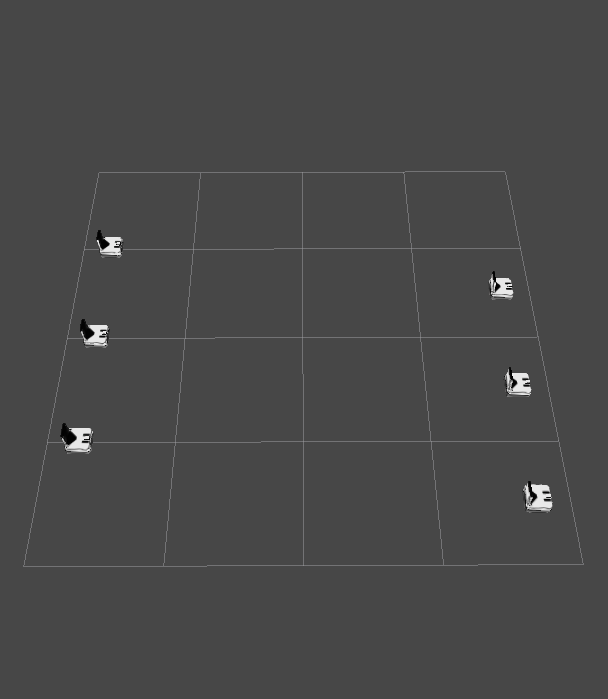
\includegraphics[width=0.24\linewidth]{figs/scene_0_0}
    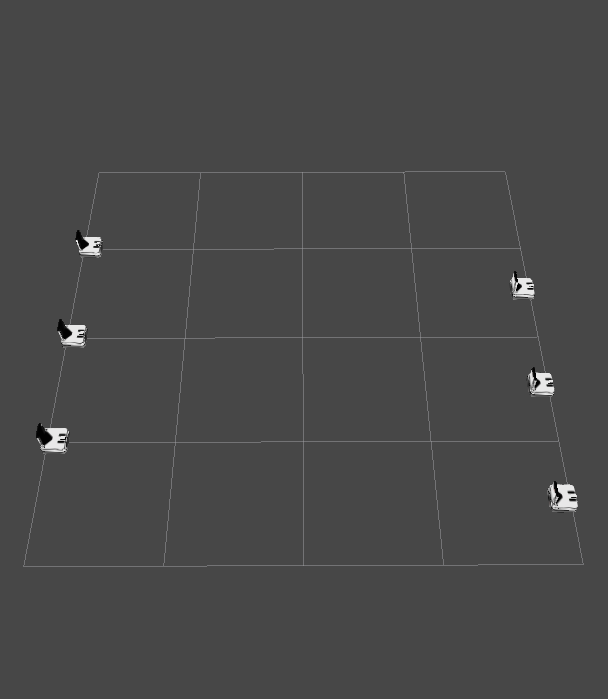
\includegraphics[width=0.24\linewidth]{figs/scene_0_1}
    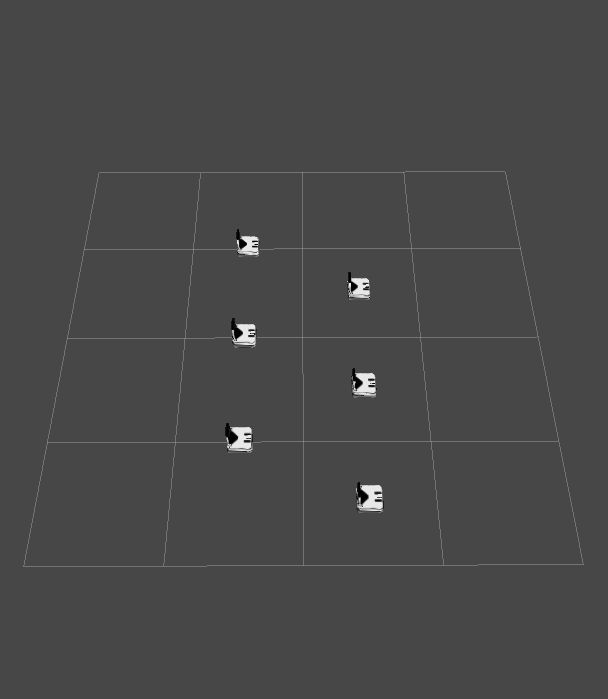
\includegraphics[width=0.24\linewidth]{figs/scene_0_2}
    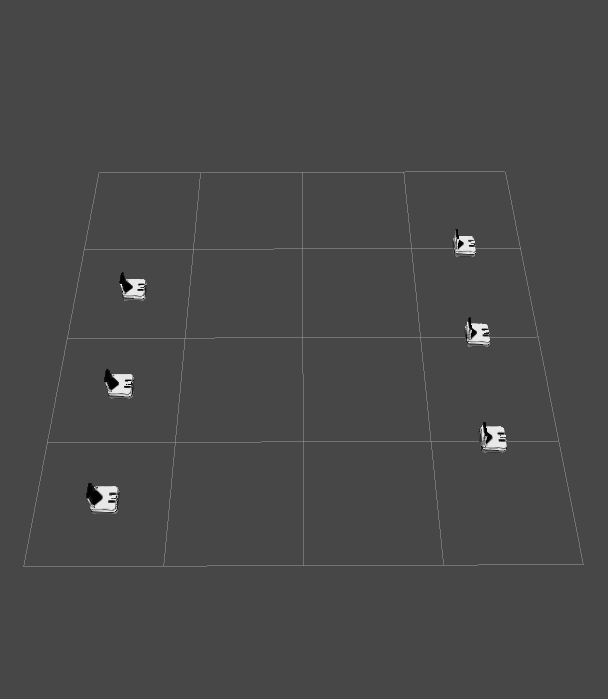
\includegraphics[width=0.24\linewidth]{figs/scene_0_3} \\
    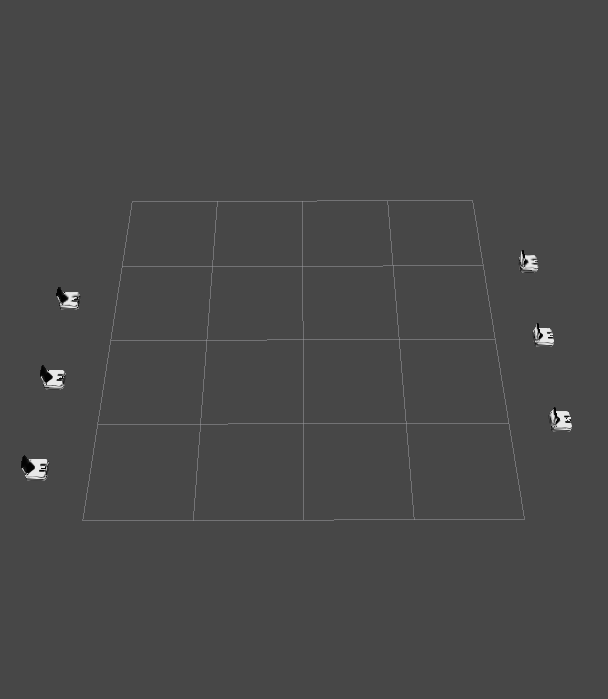
\includegraphics[width=0.24\linewidth]{figs/scene_0_4}
    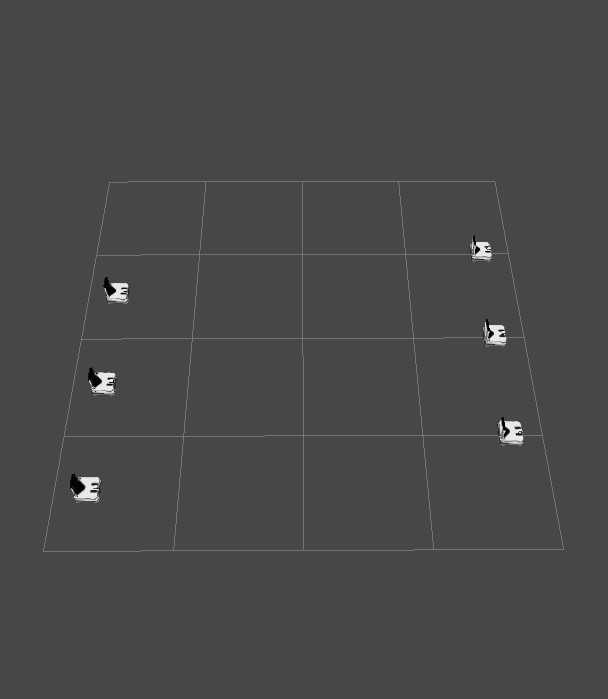
\includegraphics[width=0.24\linewidth]{figs/scene_0_5}
    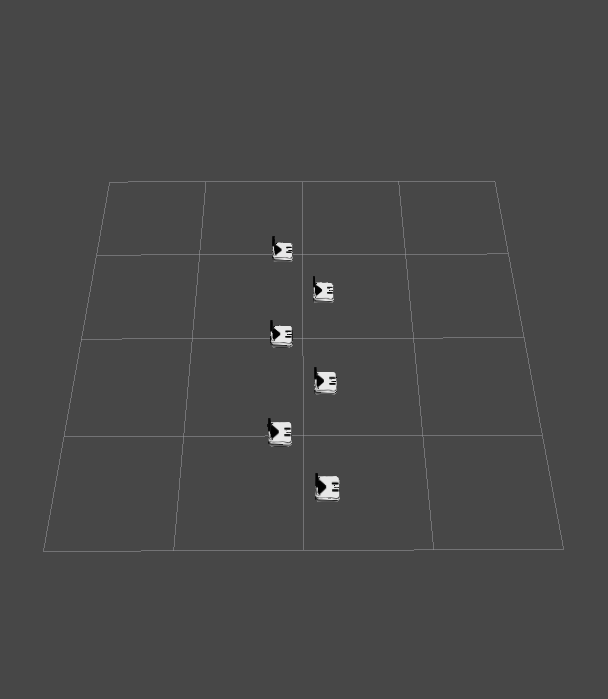
\includegraphics[width=0.24\linewidth]{figs/scene_0_6}
    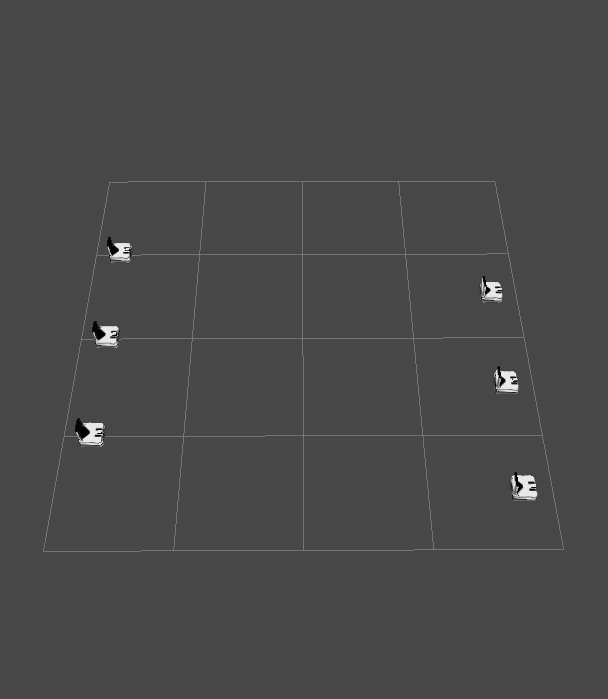
\includegraphics[width=0.24\linewidth]{figs/scene_0_7} \\
    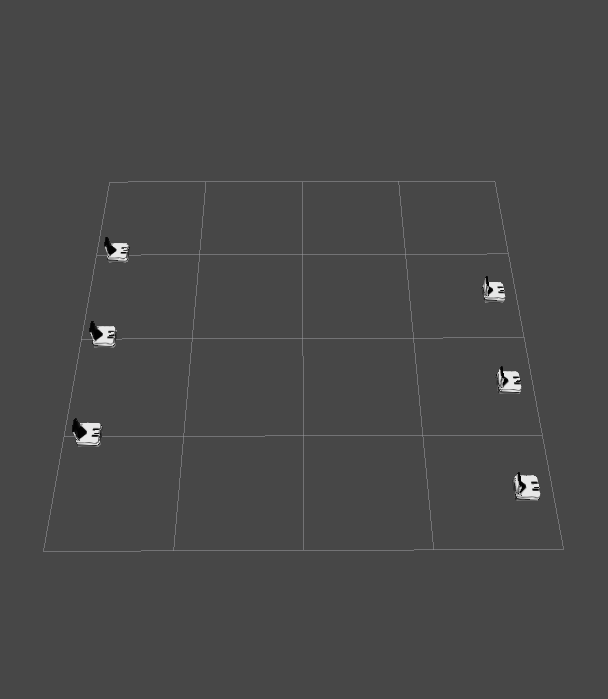
\includegraphics[width=0.24\linewidth]{figs/scene_0_8}
    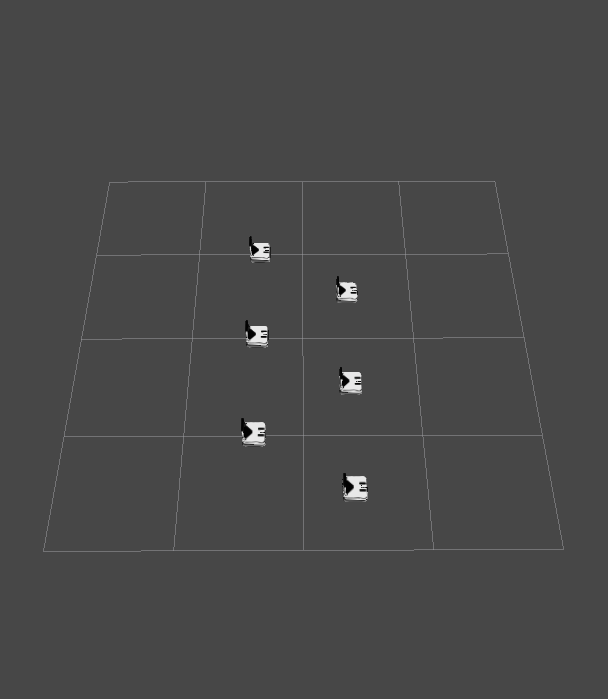
\includegraphics[width=0.24\linewidth]{figs/scene_0_9}
    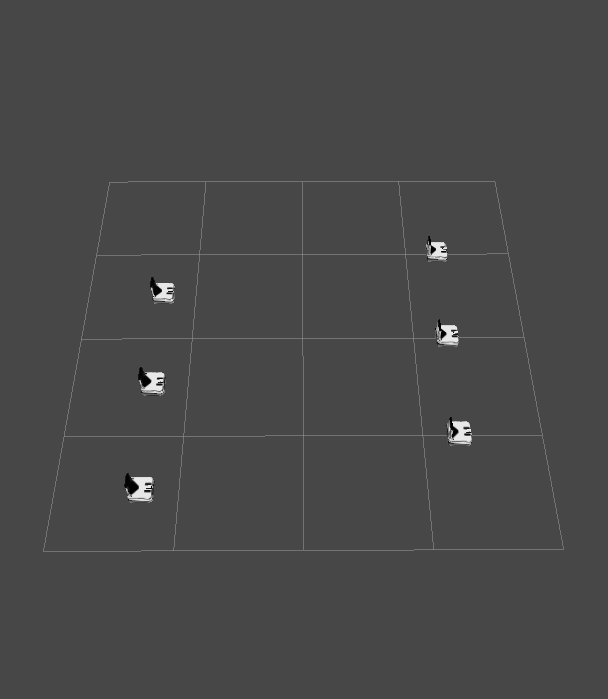
\includegraphics[width=0.24\linewidth]{figs/scene_0_10}
    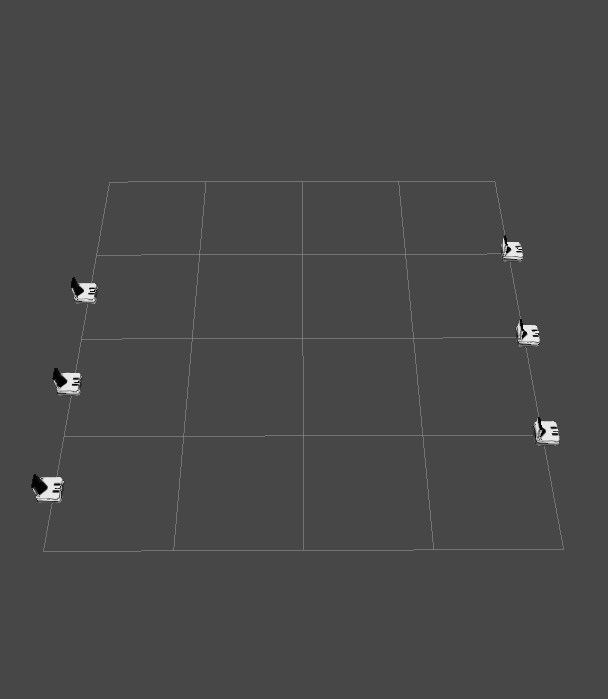
\includegraphics[width=0.24\linewidth]{figs/scene_0_11} \\
    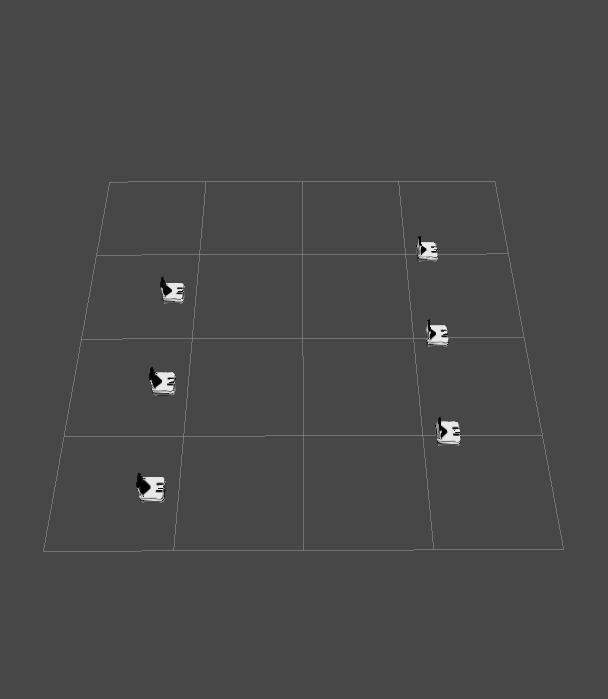
\includegraphics[width=0.24\linewidth]{figs/scene_0_12}
    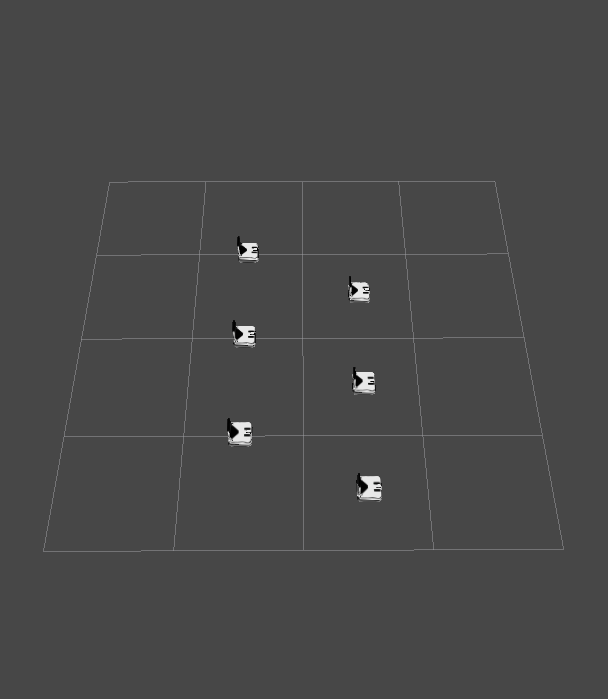
\includegraphics[width=0.24\linewidth]{figs/scene_0_13}
    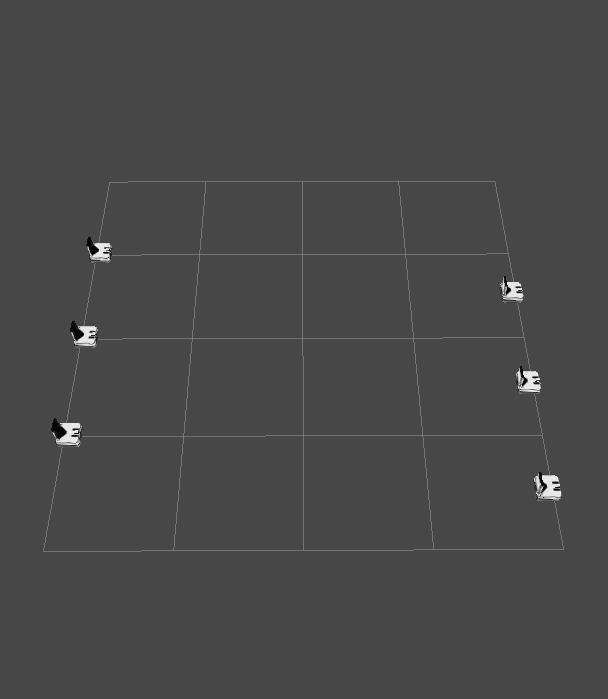
\includegraphics[width=0.24\linewidth]{figs/scene_0_14}
    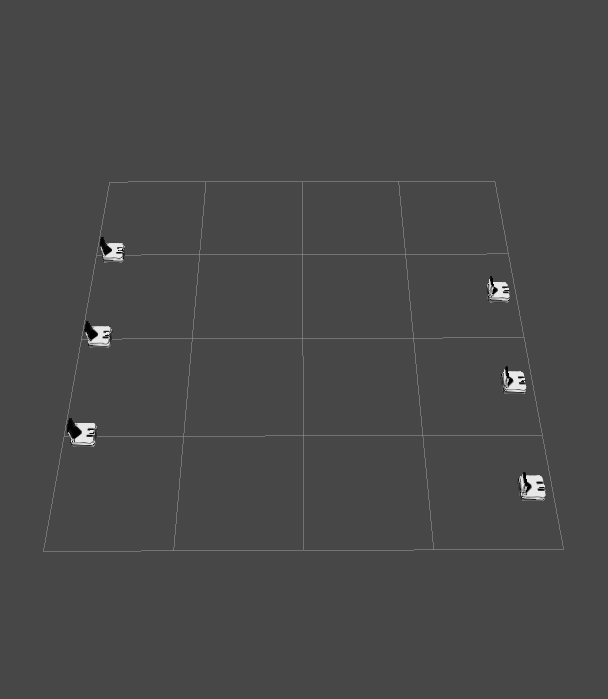
\includegraphics[width=0.24\linewidth]{figs/scene_0_15}

    \caption{A depiction of how the dynamic obstacles progress over time for
    Scene 1. No noise is added to their trajectories in order to display the
pure velocity function used for their motion. The sequences progresses from
left to right, top to bottom.}

    \label{fig:scene_0}

\end{figure}

\begin{figure}

    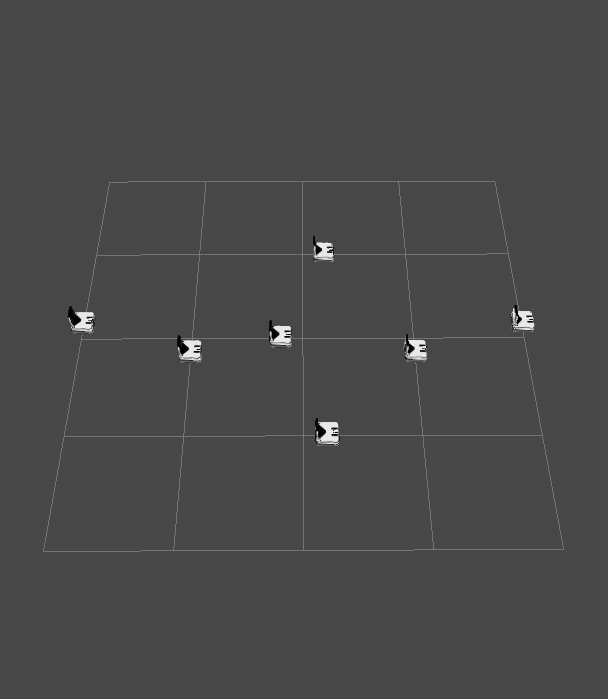
\includegraphics[width=0.24\linewidth]{figs/scene_1_0}
    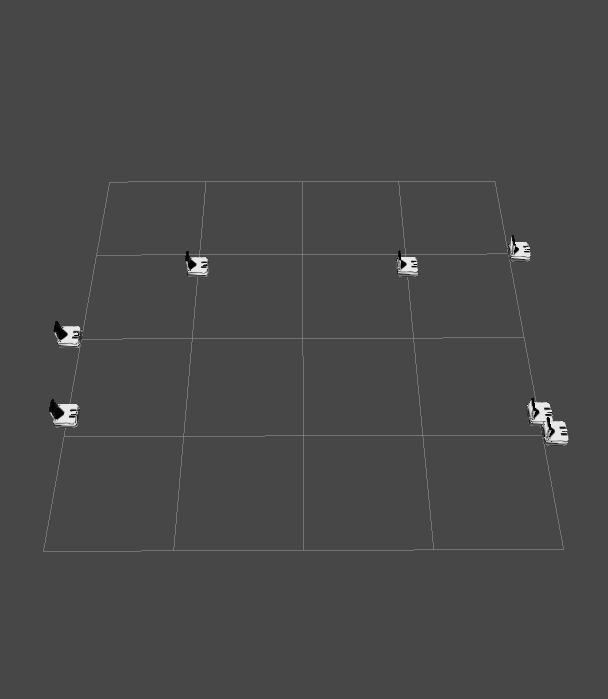
\includegraphics[width=0.24\linewidth]{figs/scene_1_1}
    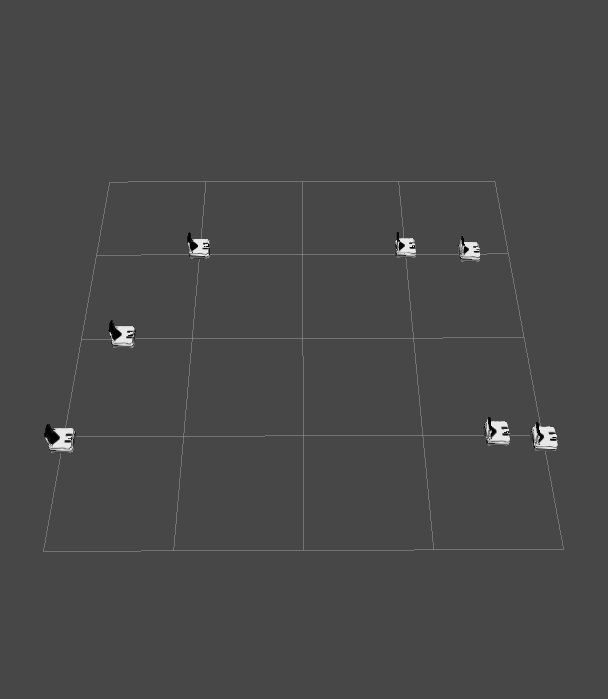
\includegraphics[width=0.24\linewidth]{figs/scene_1_2}
    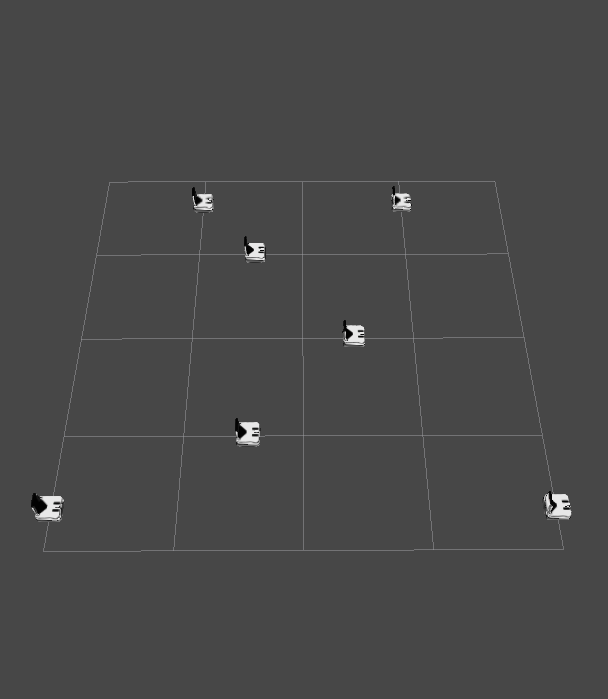
\includegraphics[width=0.24\linewidth]{figs/scene_1_3} \\
    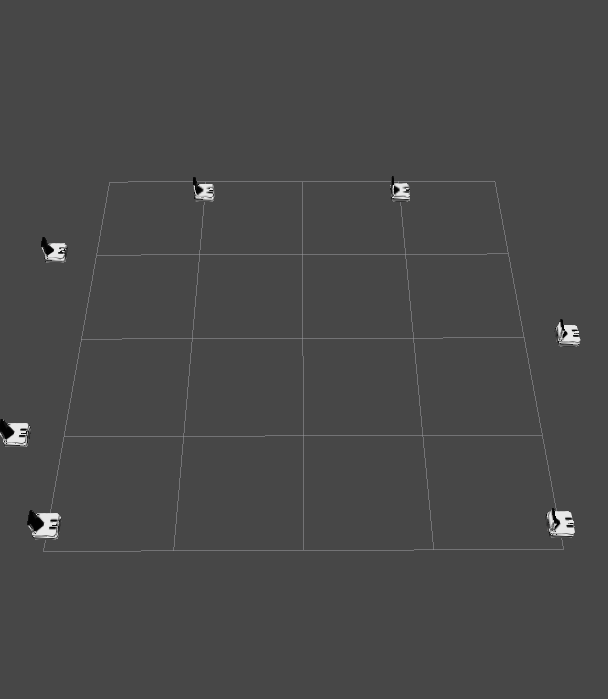
\includegraphics[width=0.24\linewidth]{figs/scene_1_4}
    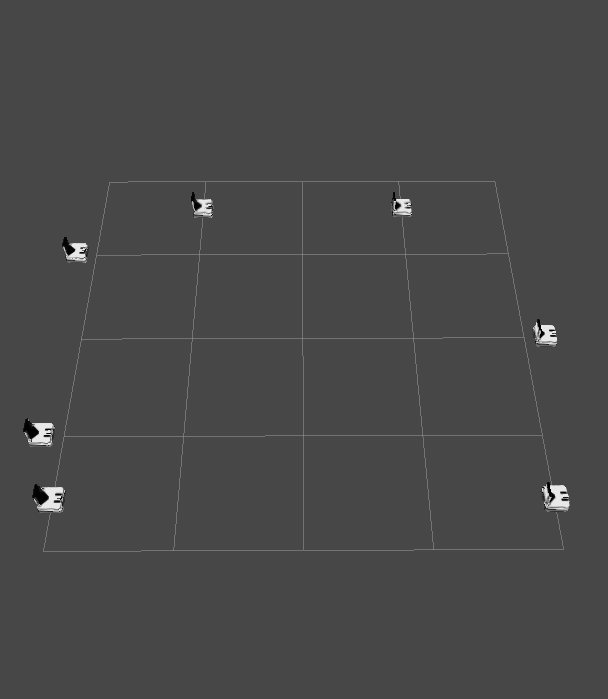
\includegraphics[width=0.24\linewidth]{figs/scene_1_5}
    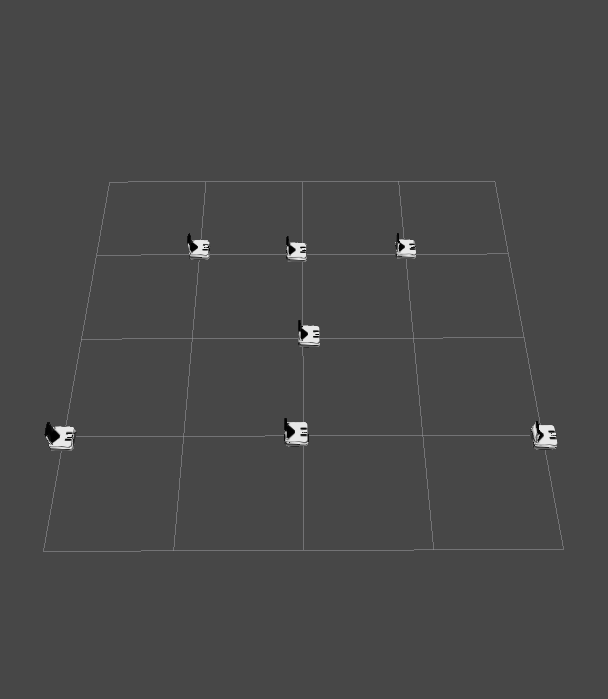
\includegraphics[width=0.24\linewidth]{figs/scene_1_6}
    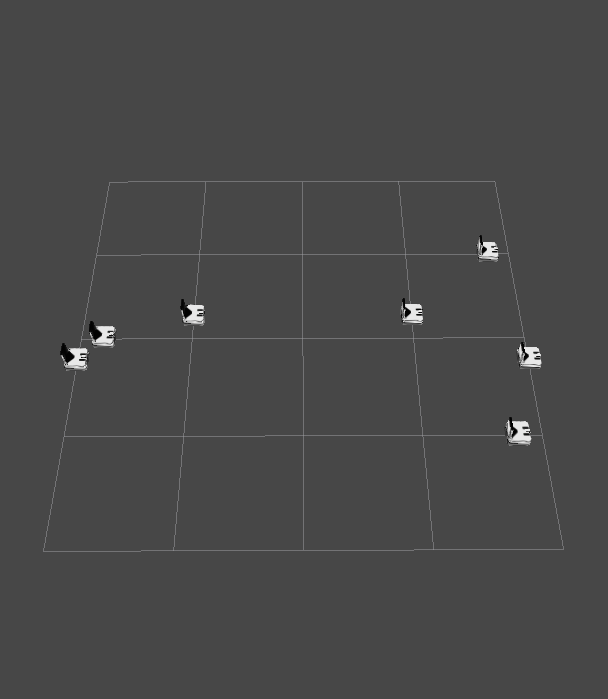
\includegraphics[width=0.24\linewidth]{figs/scene_1_7} \\
    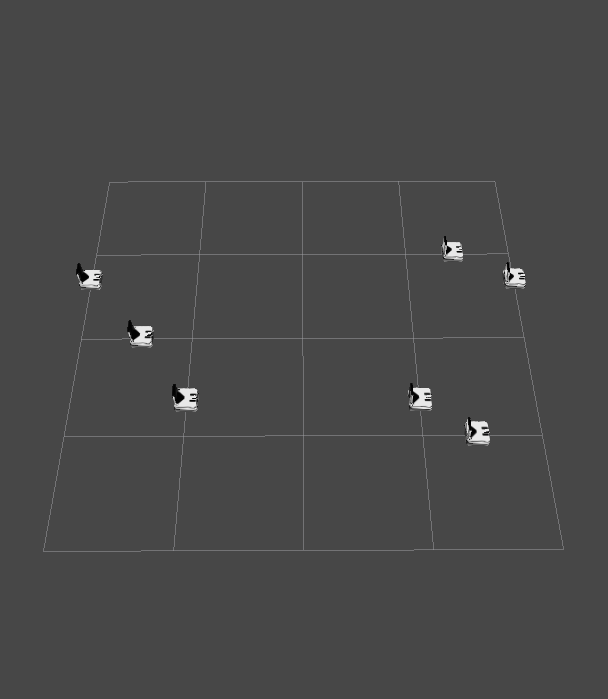
\includegraphics[width=0.24\linewidth]{figs/scene_1_8}
    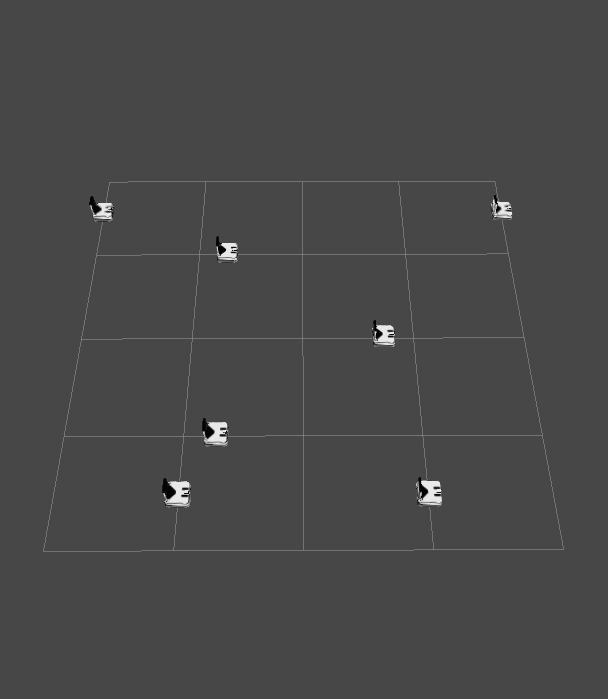
\includegraphics[width=0.24\linewidth]{figs/scene_1_9}
    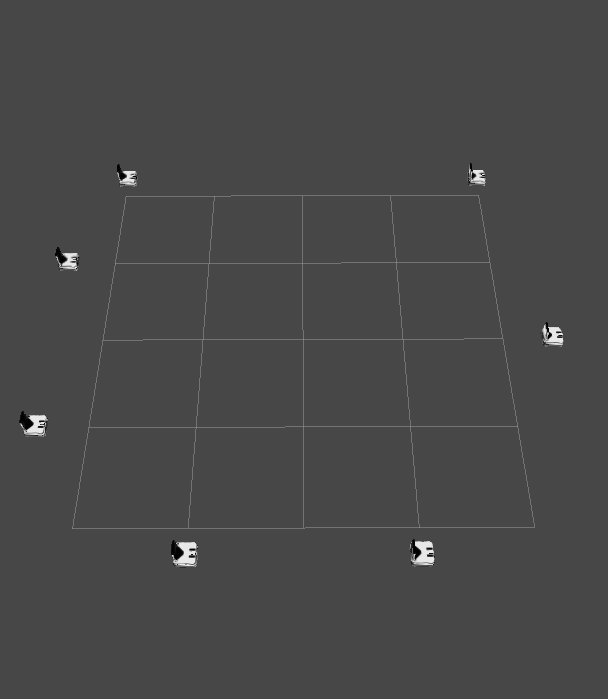
\includegraphics[width=0.24\linewidth]{figs/scene_1_10}
    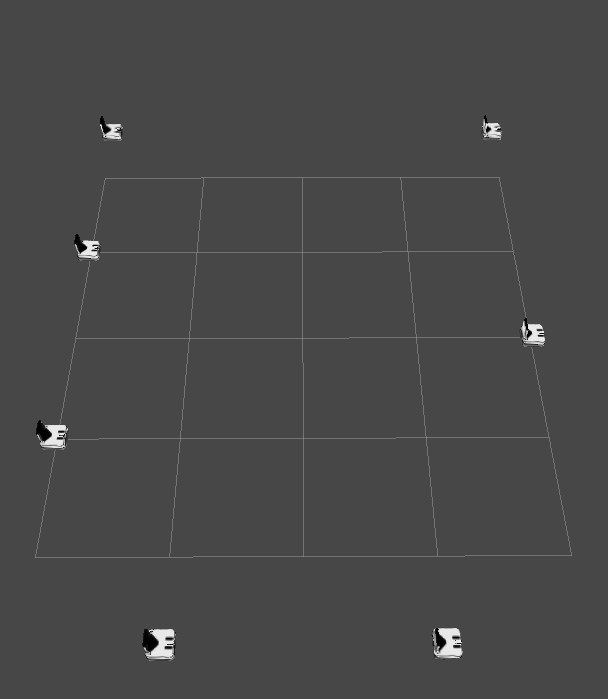
\includegraphics[width=0.24\linewidth]{figs/scene_1_11} \\
    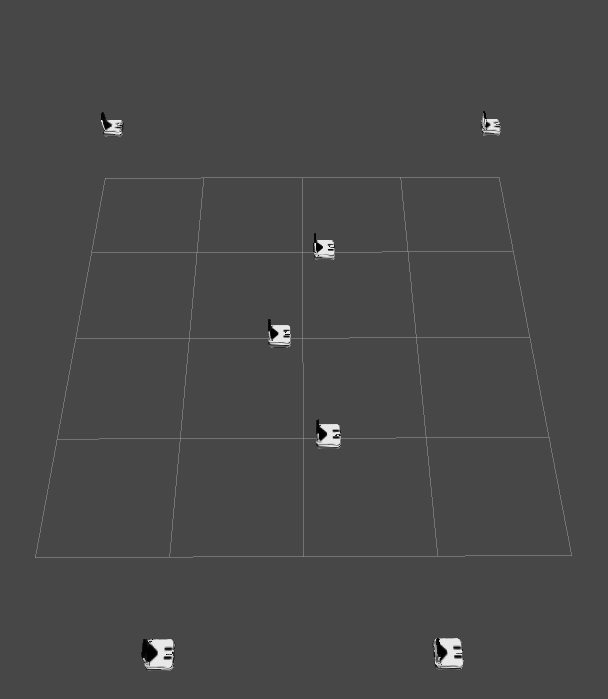
\includegraphics[width=0.24\linewidth]{figs/scene_1_12}
    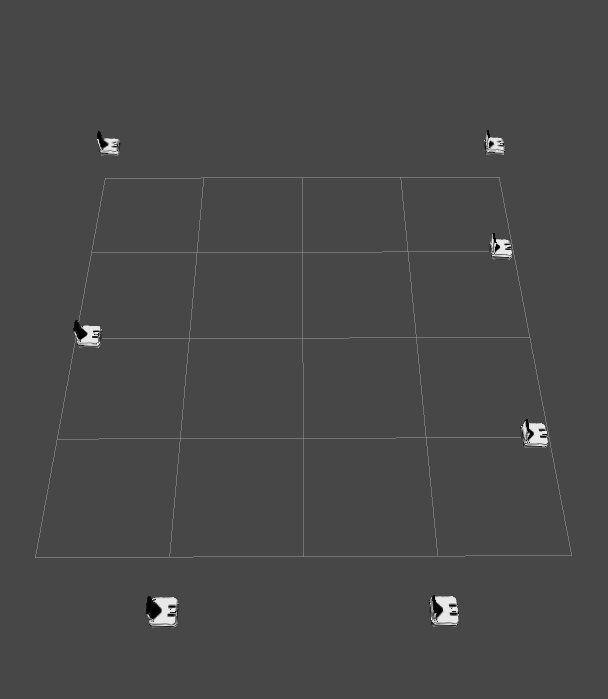
\includegraphics[width=0.24\linewidth]{figs/scene_1_13}
    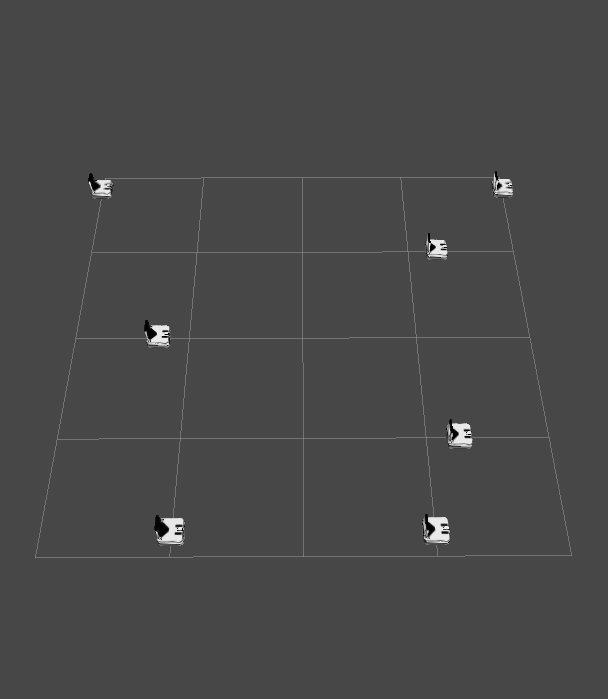
\includegraphics[width=0.24\linewidth]{figs/scene_1_14}
    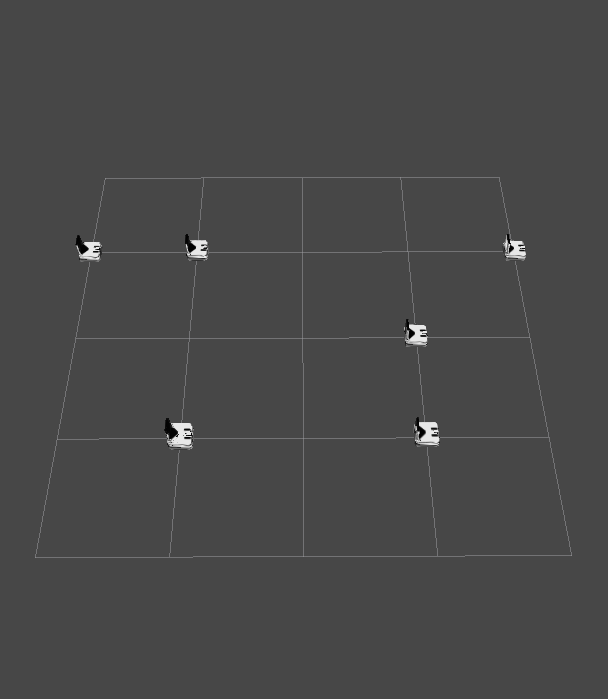
\includegraphics[width=0.24\linewidth]{figs/scene_1_15}

    \caption{A depiction of how the dynamic obstacles progress over time for
    Scene 2. No noise is added to their trajectories in order to display the
pure velocity function used for their motion. The sequences progresses from
left to right, top to bottom.}

    \label{fig:scene_1}

\end{figure}

\begin{figure}

    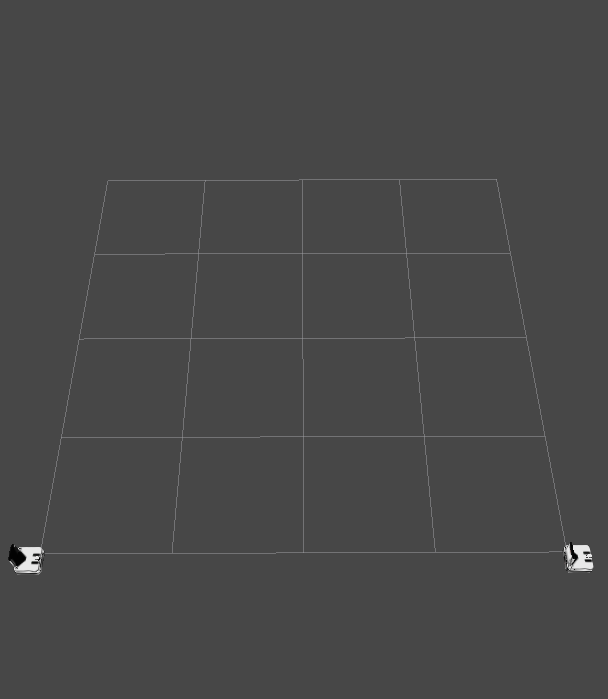
\includegraphics[width=0.24\linewidth]{figs/scene_2_0}
    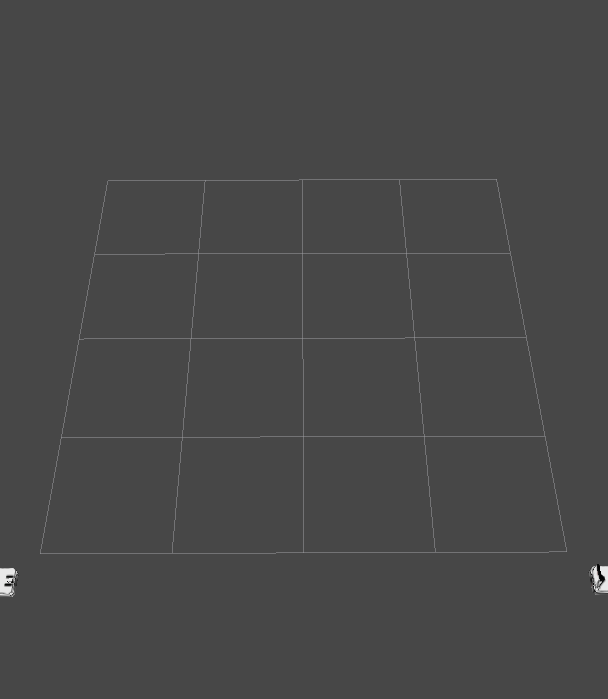
\includegraphics[width=0.24\linewidth]{figs/scene_2_1}
    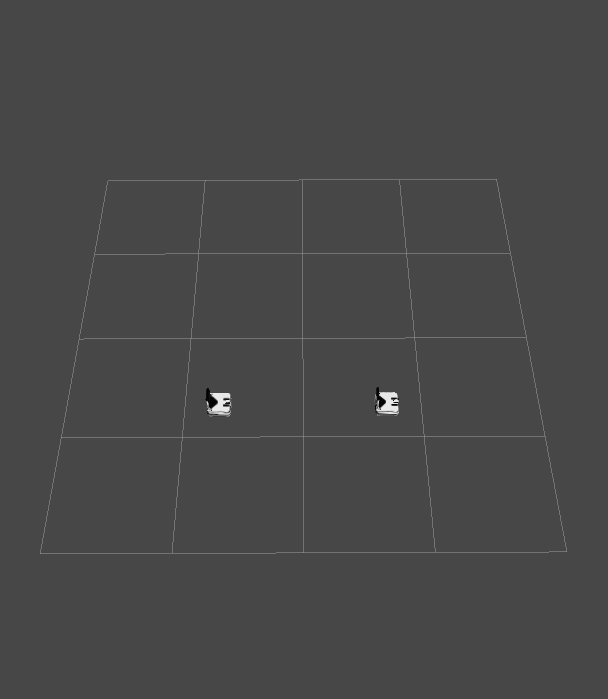
\includegraphics[width=0.24\linewidth]{figs/scene_2_2}
    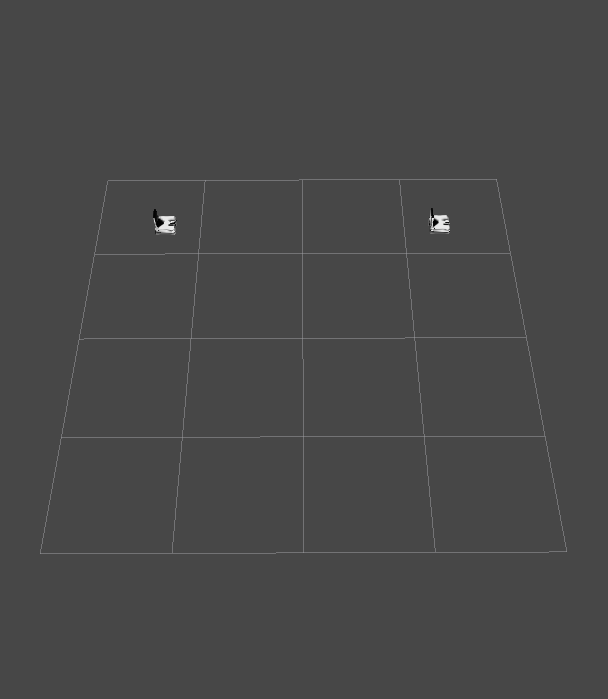
\includegraphics[width=0.24\linewidth]{figs/scene_2_3} \\
    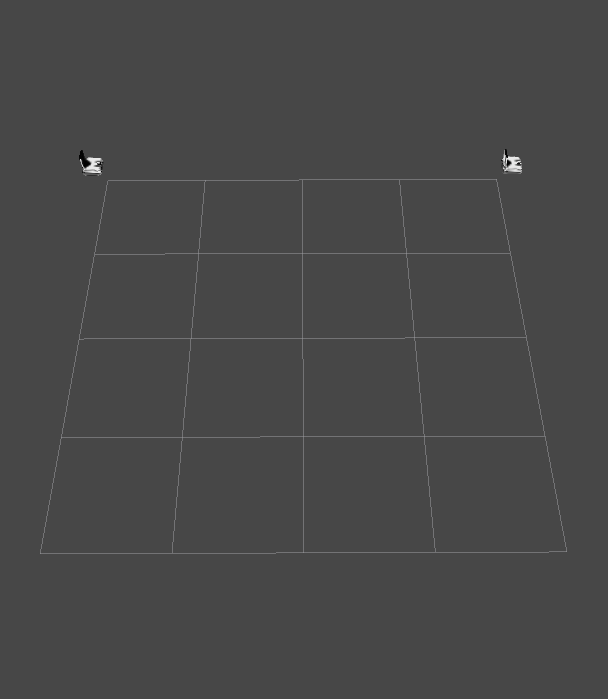
\includegraphics[width=0.24\linewidth]{figs/scene_2_4}
    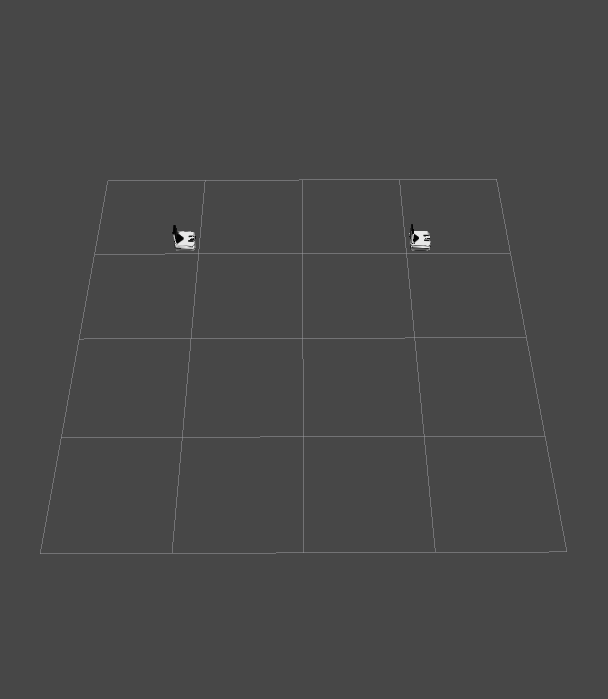
\includegraphics[width=0.24\linewidth]{figs/scene_2_5}
    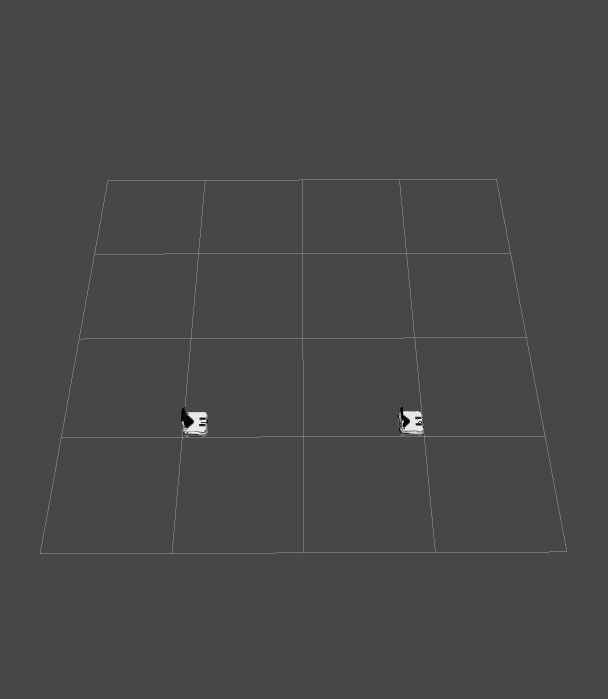
\includegraphics[width=0.24\linewidth]{figs/scene_2_6}
    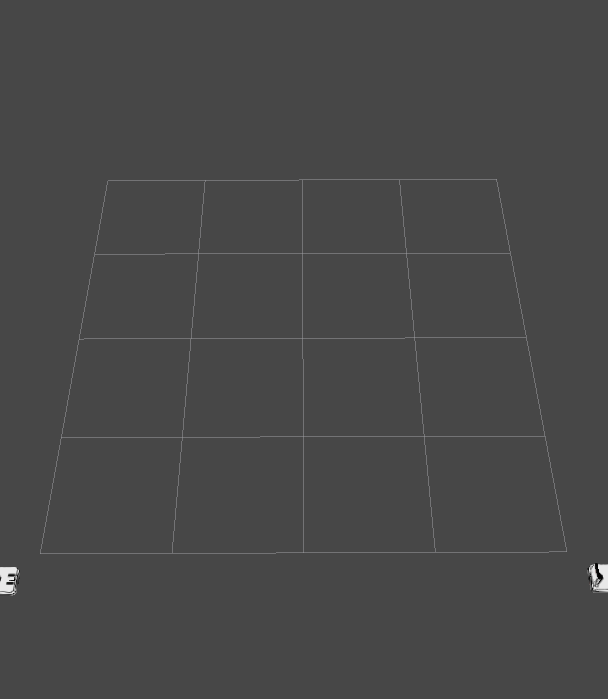
\includegraphics[width=0.24\linewidth]{figs/scene_2_7} \\
    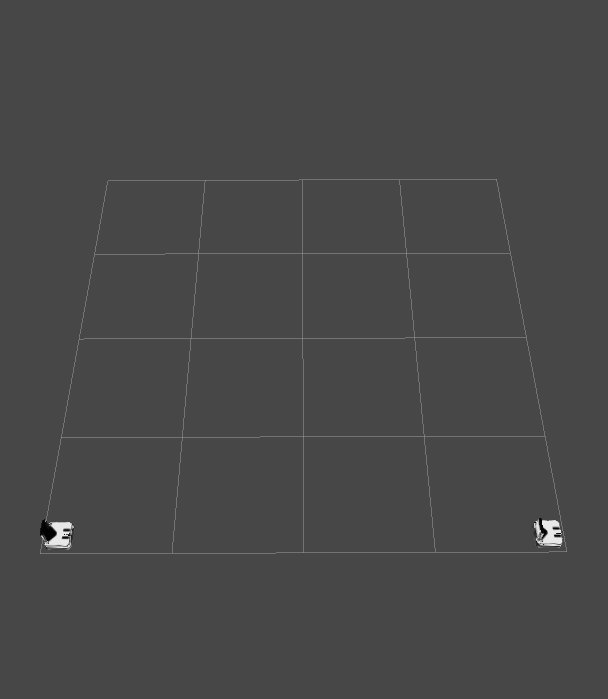
\includegraphics[width=0.24\linewidth]{figs/scene_2_8}
    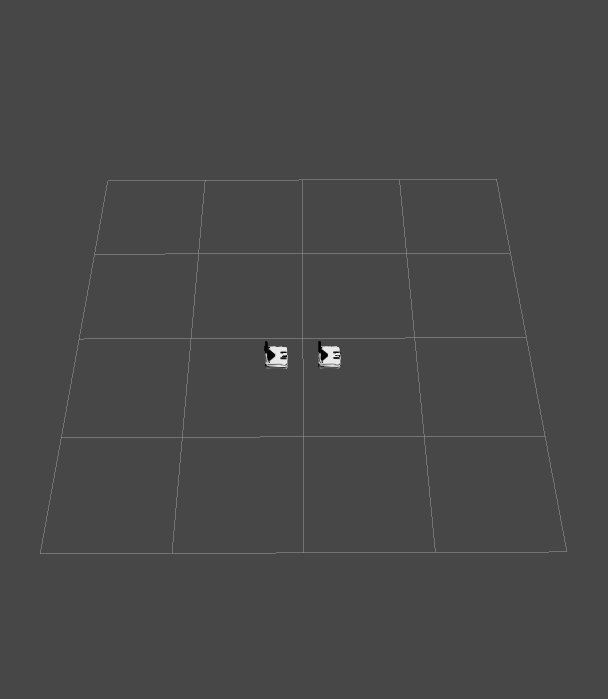
\includegraphics[width=0.24\linewidth]{figs/scene_2_9}
    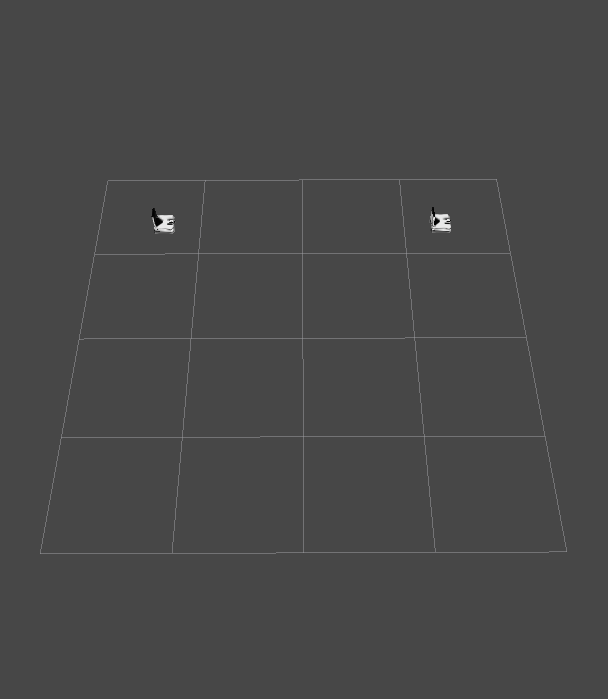
\includegraphics[width=0.24\linewidth]{figs/scene_2_10}
    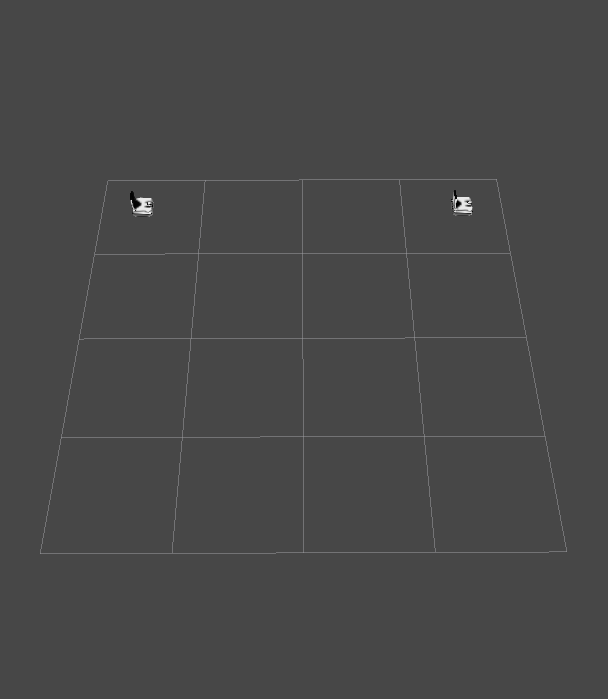
\includegraphics[width=0.24\linewidth]{figs/scene_2_11} \\
    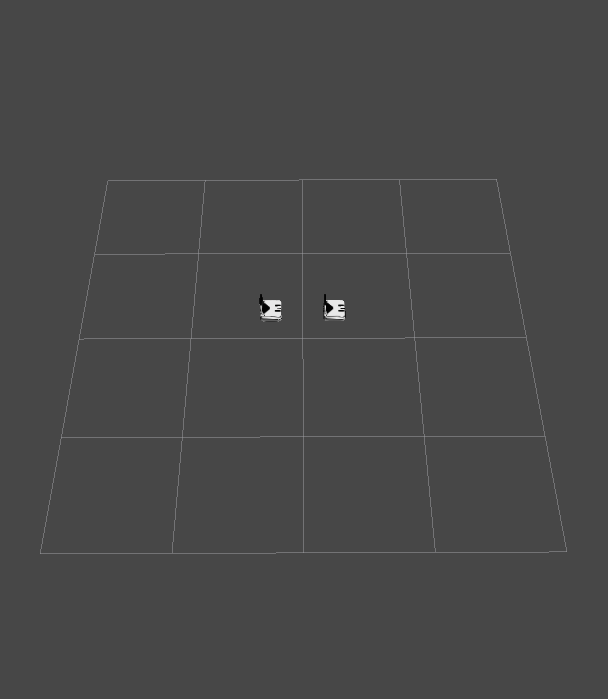
\includegraphics[width=0.24\linewidth]{figs/scene_2_12}
    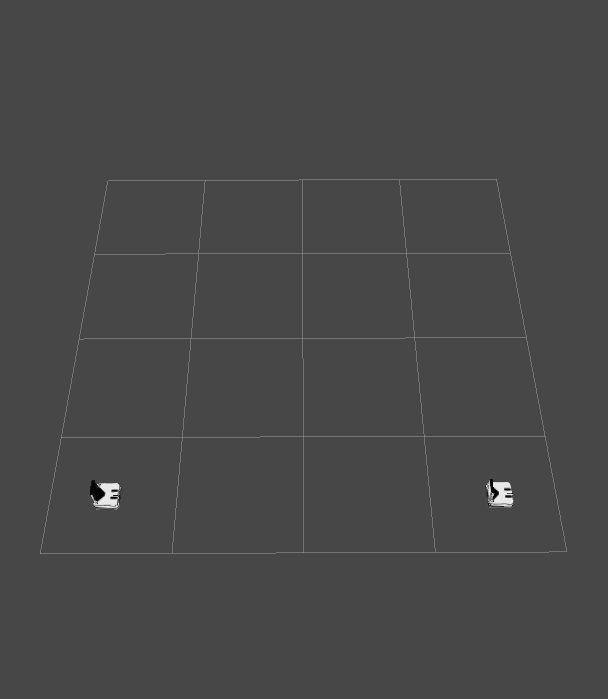
\includegraphics[width=0.24\linewidth]{figs/scene_2_13}
    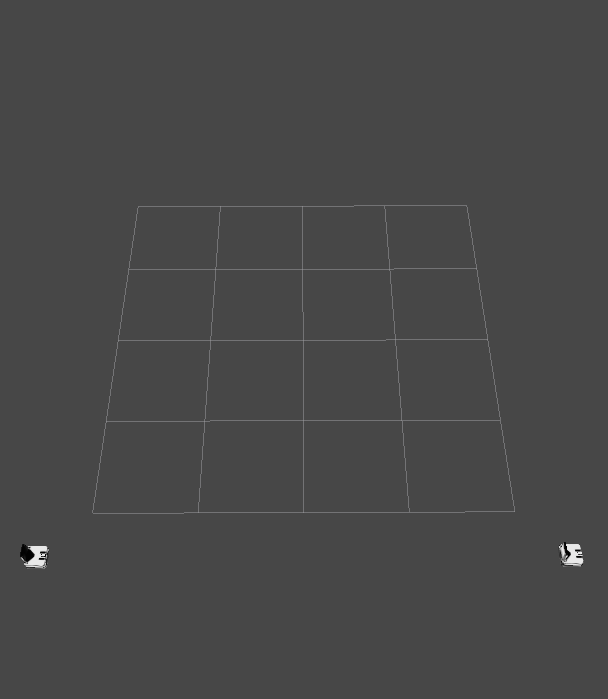
\includegraphics[width=0.24\linewidth]{figs/scene_2_14}
    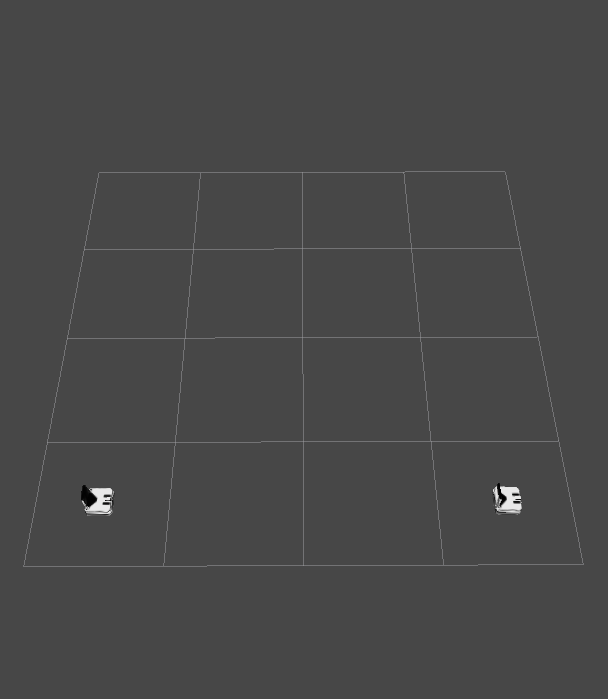
\includegraphics[width=0.24\linewidth]{figs/scene_2_15}

    \caption{A depiction of how the dynamic obstacles progress over time for
    Scene 3. No noise is added to their trajectories in order to display the
pure velocity function used for their motion. The sequences progresses from
left to right, top to bottom.}

    \label{fig:scene_2}

\end{figure}

\end{document}
